\documentclass[tikz]{standalone}
\usetikzlibrary{calc,patterns,angles,quotes}
\usepackage{pgfplots}
\pgfplotsset{compat=newest}

\pagestyle{empty}

\begin{document}
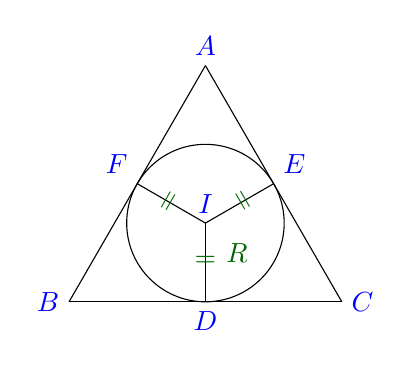
\begin{tikzpicture}
  \draw (0, 0) circle(1);
  \coordinate [label={[blue]above:$A$}] (A) at (0, 2);
  \coordinate [label={[blue]right:$C$}] (C) at (1.732, -1);
  \coordinate [label={[blue]left:$B$}] (B) at (-1.732, -1);
  \coordinate [label={[blue]above:$I$}] (I) at (0, 0);
  \coordinate [label={[blue]below:$D$}] (D) at (0, -1);
  \coordinate [label={[blue]above right:$E$}] (E) at (.866, 0.5);
  \coordinate [label={[blue]above left:$F$}] (F) at (-.866, 0.5);
  \draw (B) -- (C);
  \draw (A) -- (B);
  \draw (C) -- (A);
  \draw (I) -- (D);
  \draw (I) -- (E);
  \draw (I) -- (F);
  \coordinate [label={[label distance=0.2cm, black!60!green] below right:$R$}] (A2) at (0, 0);
  \node[label={[black!60!green, yshift=-0.3cm]:$=$}] at (0, -.5 ) (A1) {};
  \node[label={[black!60!green, rotate=120, yshift=-.2cm, xshift=-0.1cm]:$=$}] at ( $ (E)!0.5!(I) $ ) (C1) {};
  \node[label={[black!60!green, rotate=240, yshift=-.2cm, xshift=0.1cm]:$=$}] at ( $ (F)!0.5!(I) $ ) (B1) {};
\end{tikzpicture}
\end{document}
